\documentclass[conference]{IEEEtran}
\IEEEoverridecommandlockouts
% The preceding line is only needed to identify funding in the first footnote. If that is unneeded, please comment it out.
\usepackage{cite}
\usepackage{amsmath,amssymb,amsfonts}
\usepackage{algorithmic}
\usepackage{graphicx}
\usepackage{textcomp}
\usepackage{xcolor}
\def\BibTeX{{\rm B\kern-.05em{\sc i\kern-.025em b}\kern-.08em
    T\kern-.1667em\lower.7ex\hbox{E}\kern-.125emX}}
\begin{document}

\title{Experimental investigation of forced convective heat transfer in cylindrical pipe flow\\
%{\footnotesize \textsuperscript{*}Note: Sub-titles are not captured in Xplore and should not be used}
%\thanks{Identify applicable funding agency here. If none, delete this.}
}

\author{\IEEEauthorblockN{Yoshinori Hattori}
\IEEEauthorblockA{\textit{Shibaura Institute of Technology, Mechanical Engineering}\\
Tokyo, Japan \\
%\textit{Graz University of Technology, Institute of Fluid Mechanics and Heat Transfer}\\
%Graz, Austria \\
md18060@shibaura-it.ac.jp}}

\maketitle

%\begin{abstract}
%This document is a model and instructions for \LaTeX.
%This and the IEEEtran.cls file define the components of your paper [title, text, heads, etc.]. *CRITICAL: Do Not Use Symbols, Special Characters, Footnotes,
%or Math in Paper Title or Abstract.
%\end{abstract}

\begin{IEEEkeywords}
Forced convection, Nusselt number, Wall friction, transitional, Cylindrical pipe flow
\end{IEEEkeywords}

\section{Introduction}
Forced convective heat transfer in cylindrical pipe flow plays an important role in many technical cooling systems.
These coolant technology is used wide varaety of coolant applications such as electric devices, automotive, and plant factry.
Considering heat transfer issues, heat transfer coefficient is one of the most important numbers.

Much remains to be studied for providing experimental data for high Pramblt number and laminar-to-turbulent transitional regime.
In this paper, we focus on forced convective heat transfer in cylindrical pipe flow in particular high Pramblt number and transitional regime.
%The experiment was carried out considering a board range of Reynolds number, spanning from laminar to fully turbulent flow.
A 50/50vol\% mixture of water and glycole which is a typical liquid coolant in automotive applications were used as a operating fluid.
This coolant liquid is normally used in low temperature.
However, it's difficult to maintain the cylindical pipe at low temperature.
Therefore, as a 1st approach, we take a data for high temperature and then compared with Direct numerical simulation (DNS).
If there is a good agreement between experimental data for high temperature and DNS, the result in a low temperature would be predicted by DNS.
%In this paper we apply the techniques of Laser-induced fluorescence (LIF) to find out temperature distribution in cylindrical pipe flow.
Moreover, the investigation shall also include the measurement of wall friction coefficient.
The engineeres is frequently interested in pressure drop which is related to determine pump or fan power equipments.
The experimental data compared with some correlations and other sources as well as computational results obtained from already existing numerical simulations (CFD) by Rorenzo\cite{Rorenzo2019}.

\section{The phenomena}
%%Temperature variations for constantHeat flux
%\begin{figure}[htbp]
%  \centering
%  %\vspace{-3zh}
%  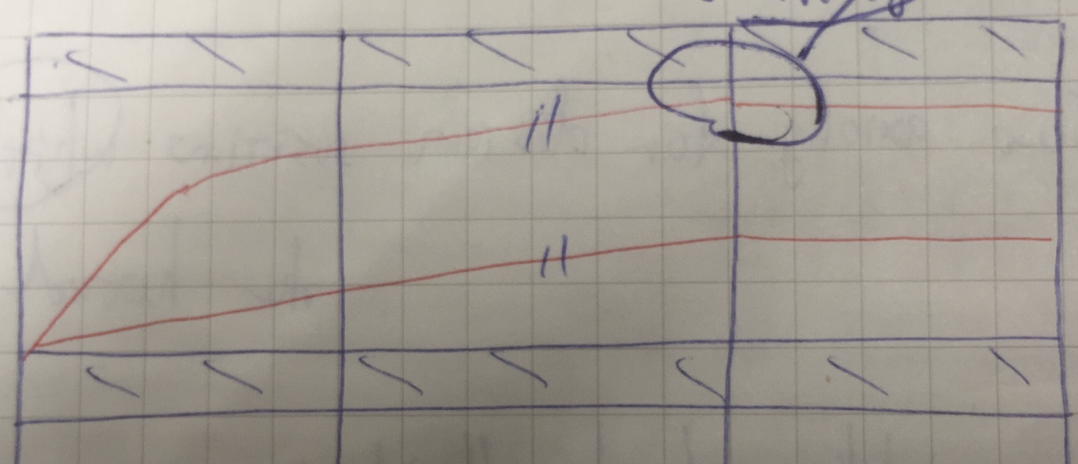
\includegraphics[width=0.47\textwidth,natwidth=610,natheight=642]{fig/temperature_variations_constant_heat_flux.png}
%  \caption{Temperature variations for constantHeat flux}
%  \label{temperature_variations_constant_heat_flux}
%\end{figure}
%
%%Heat transfer coefficient depend on x value
%Figure\label{heat_transfer_coefficient_depend_on_x_value} shows the local heat transfer coeeficient 
%\begin{figure}[htbp]
%  \centering
%  %\vspace{-3zh}
%  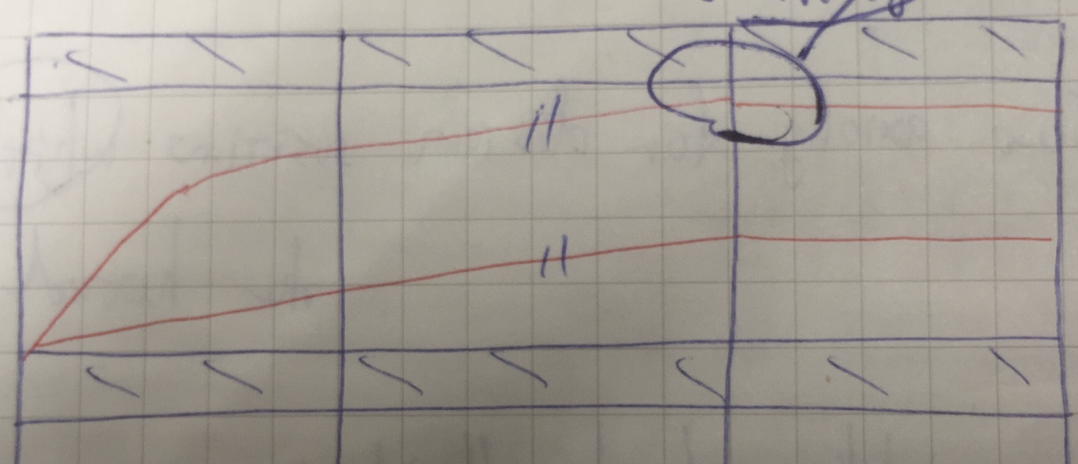
\includegraphics[width=0.47\textwidth,natwidth=610,natheight=642]{fig/temperature_variations_constant_heat_flux.png}
%  \caption{Heat transfer coefficient depend on x value}
%  \label{heat_transfer_coefficient_depend_on_x_value}
%\end{figure}
%There are two surface conditions arise in many engineering applications.
%One is constant surface heat flux and the other is constant surface temperature.
%In the fully developed flow of the tube, fluid constant porperties, the local heat coefficient is constant independent of x.

\section{Experimental setup}
%Experimental Setup
The experimental setup is already existing facilities by Christphan2018 figure.() .
\begin{figure}[htbp]
  \centering
  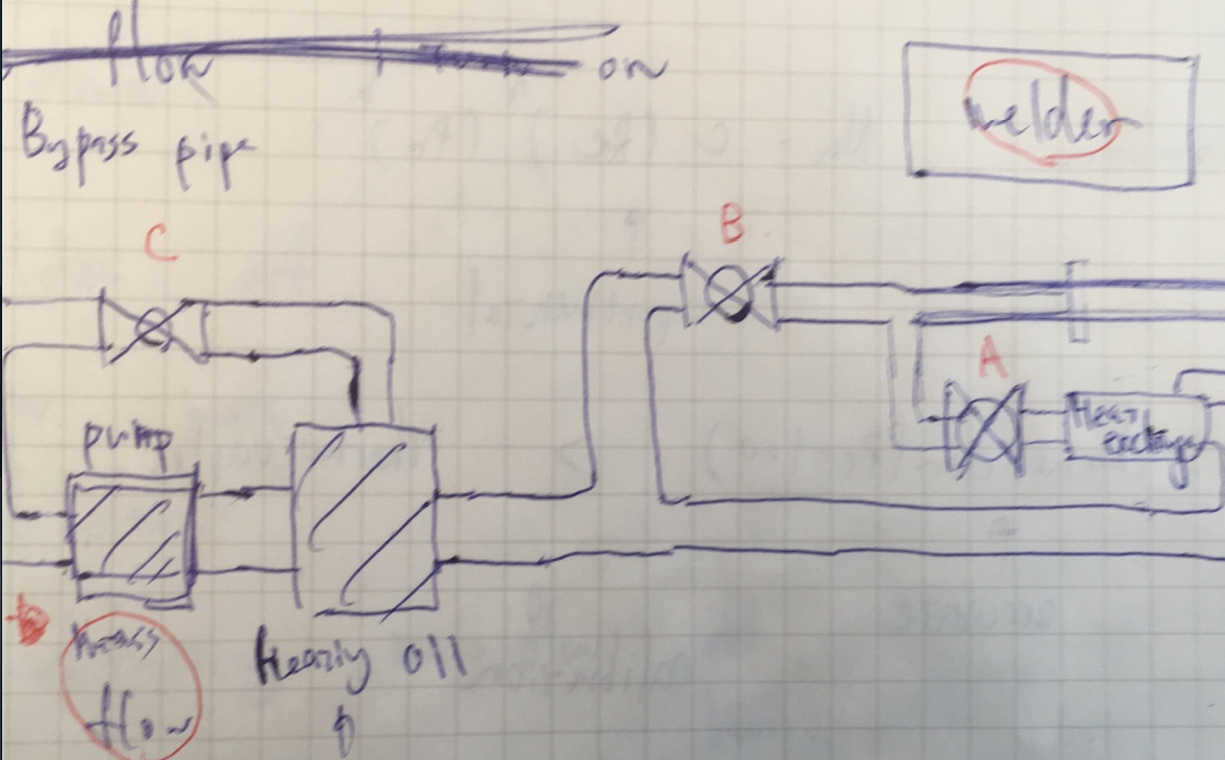
\includegraphics[width=0.47\textwidth,natwidth=610,natheight=642]{fig/experimental_setup.pdf}
  \caption{Experimental setup.}
  \label{experimental_setup}
  \vspace{-2zh}
\end{figure}
The experimental setup loop consists of heat exchanger, pump, coriolis mass flow rate, welder, reservoir, and test section basically.
Heat exchenger keep thermal stationary condition in flow pipe.
Mass flow rate is controlled by pump and baypass pipe which is located parallel.

Figure\label{thermal_boundary_layer_development} shows the tube in a test-sction area.
The test section is made of stainless steel (1.4301) with an inner diameter di=12mm and outer diameter do= 15mm.
The test section consist of entrance, heated region and thermal equalisation.
\begin{enumerate}
  \item Entrance part\\
  The first part of test section is 1.2[m] length entrance part which is sufficiently long to ensure dynamically developed flow condition at the exist.(*) The bulk temperature(Tb0) at this section were measured by PT-100.
  \item Heated part\\
  The second part of test section is 2[m] length heated part which is sufficiently long to ensure thermaly fully developed flow condition at the exist.(*) The tube wall were heated electrically by welder which provide high current and low voltage to keep the uniform heat flux condition in a inner pipe flow. The wall temperature(Tw) at the exist of this section were measured by PT-100.
  \item Thermal equalization part\\
  The third part of test section is thermall equalisation part which is including static mixture. Static mixture forms turbulent and vortex. Then, the thermal profile of heated exist mix tigether. At the end, the bulk temperature(Tb1) are measured.(Assumed that the pipe is thermal isolated, surrounded with glass wool.)
\end{enumerate}

Highly accurate resistance thermall probes (PT-100) are used to find out the inlet and outlet bulk temperature (Tib , Tob) and wall temperature Tw.
Moreover, thermocouple 'Type-K' are used to take temperature gradient in flow direction.
However, those thermocouples aren't directly related to calculete four parameters.(Re,Nu,Pr,Cf)
\begin{figure}[htbp]
  \centering
  %\vspace{-3zh}
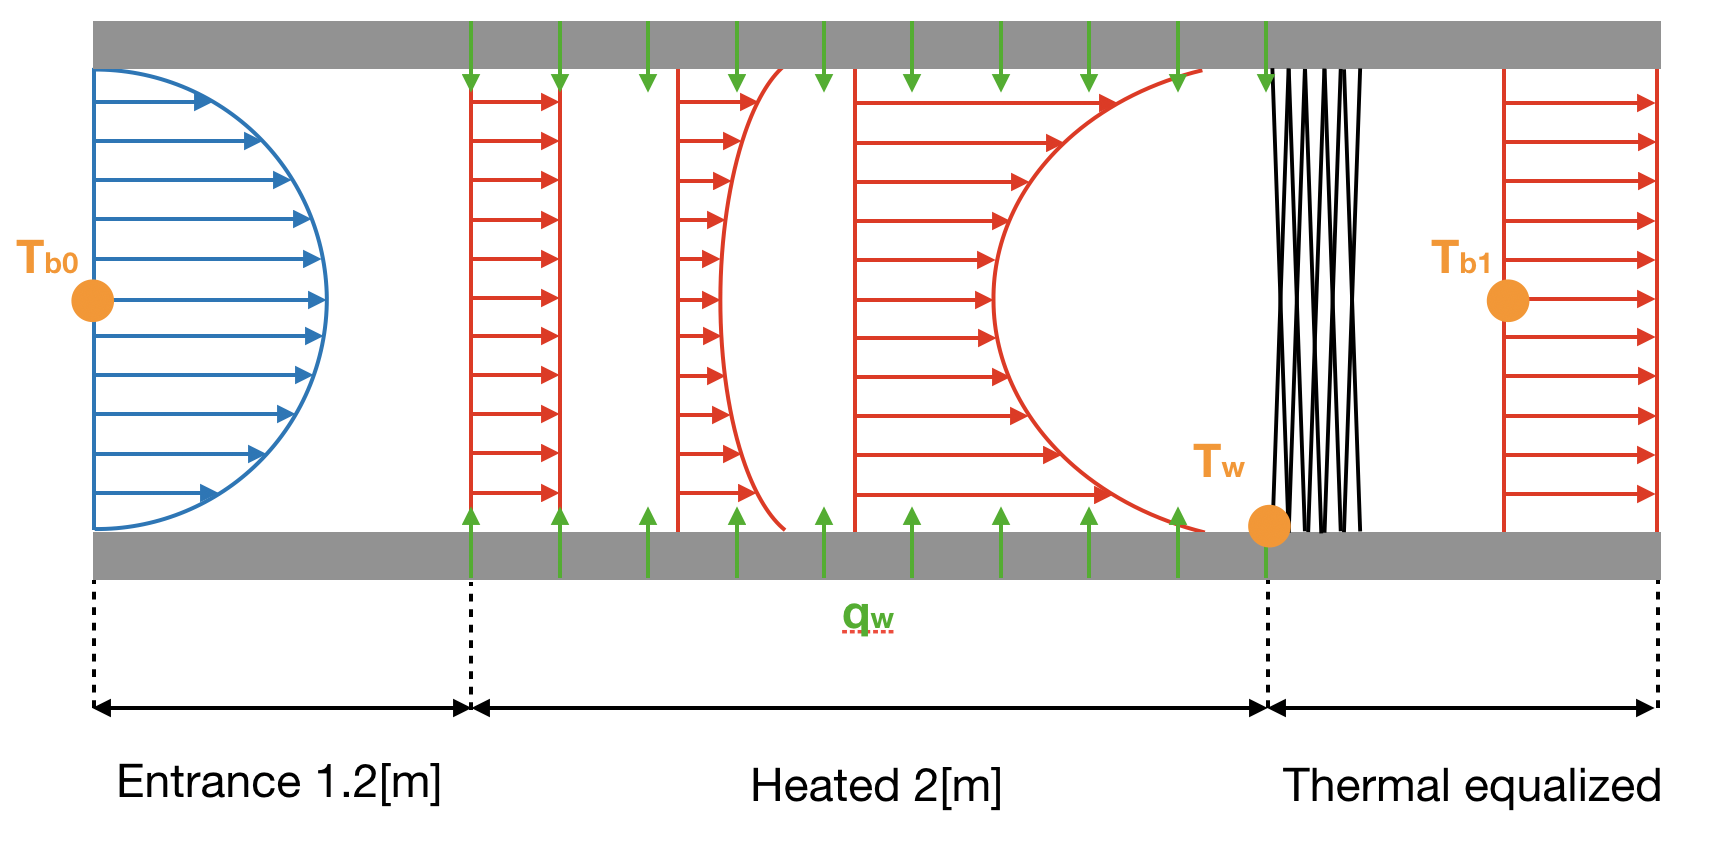
\includegraphics[width=0.47\textwidth,natwidth=610,natheight=642]{fig/thermal_boundary_layer_development.png}
  \caption{Thermal boundary layer development}
  \label{thermal_boundary_layer_development}
\end{figure}

There are 3 ways to control Re, Pr.
It is hard to keep high Pr and low Re.
Figure\label{density_rho} shows material properties of Shell Heat Transfer Oil S2.

\begin{enumerate}
  \item Cooling water\\
  As opening valve A and closing valve B, decreasing flow temperature.
  Then, viscosity increase and Re decrease and Pr increase.
  \item Bypass pipe\\
  As opening bypass pipe C, decreasing mass flow rate then, Re decrease.
  As decreasing mass flow rate, Pr decrease because the number is related to heat transfer convection from the wall. (Heat is provided from the wall.)
  In order to decrease mass flow rate, controlling bypass pipe is stronger than pump machine.
  \item Welder and mass pump machine\\
  As decreasing mass flow rate (pump machine) and welder, Re decrease and Pr nearly constant.
  Pr is proposonal to Nu which is, convection devided by conduction.
  Controlling both welder and mass flow rate, the ratio is maintained constant value.
\end{enumerate}

\begin{figure}[h]
\begin{minipage}{0.48\linewidth}
 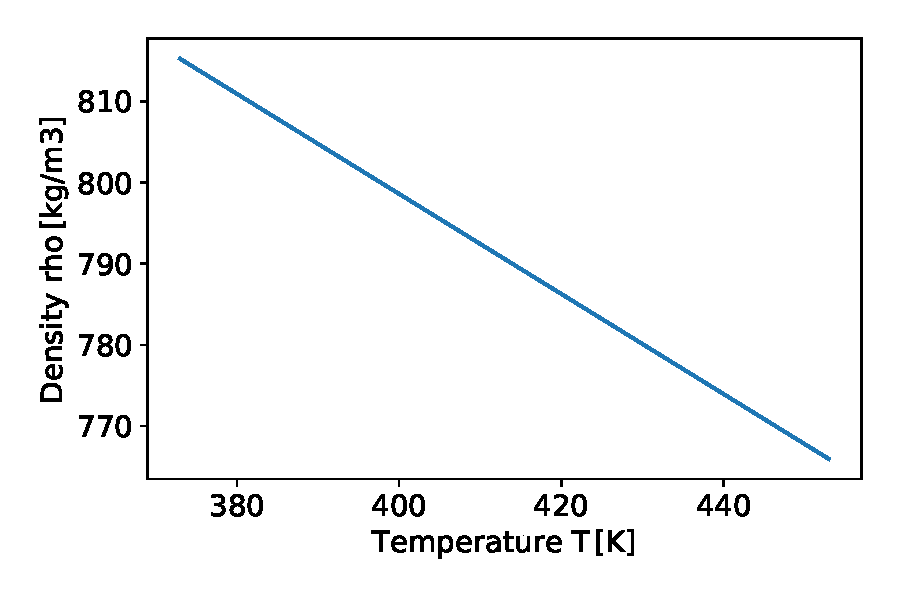
\includegraphics[width=0.48\textwidth,natwidth=190,natheight=210]{fig/density_rho.pdf}
 \vspace{-1zh}
 \caption{Density rho, $\rm kg/m^{3}$}\label{density_rho}
\end{minipage}
\hfill
\begin{minipage}{0.48\linewidth}
 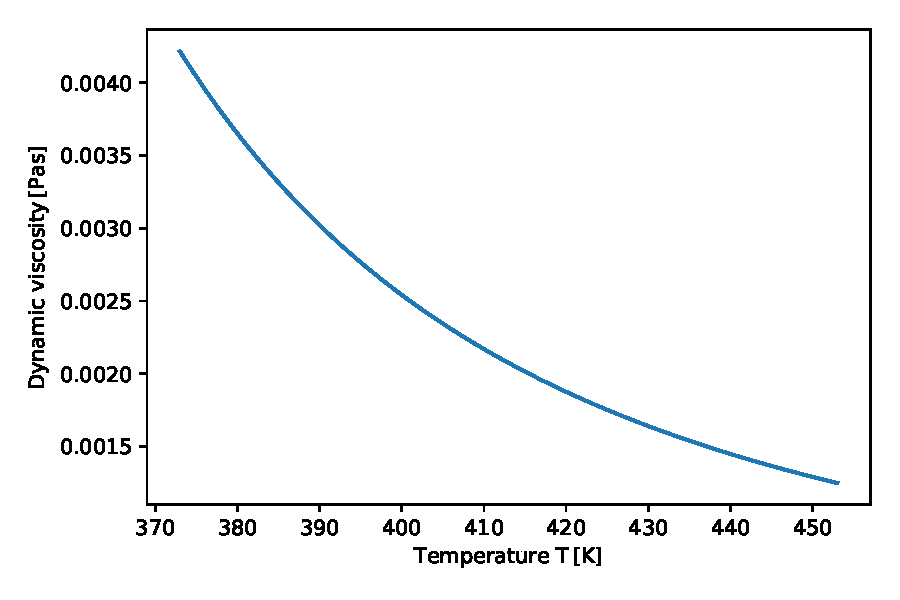
\includegraphics[width=0.48\textwidth,natwidth=190,natheight=210]{fig/dynamic_viscosity.pdf}
 \vspace{-1zh}
 \caption{Dynamic viscosity mu, $\rm Pa s$}\label{dynamic_viscosity}
\end{minipage}
\vspace{2zh}
\end{figure}

\begin{figure}[h]
\begin{minipage}{0.48\linewidth}
 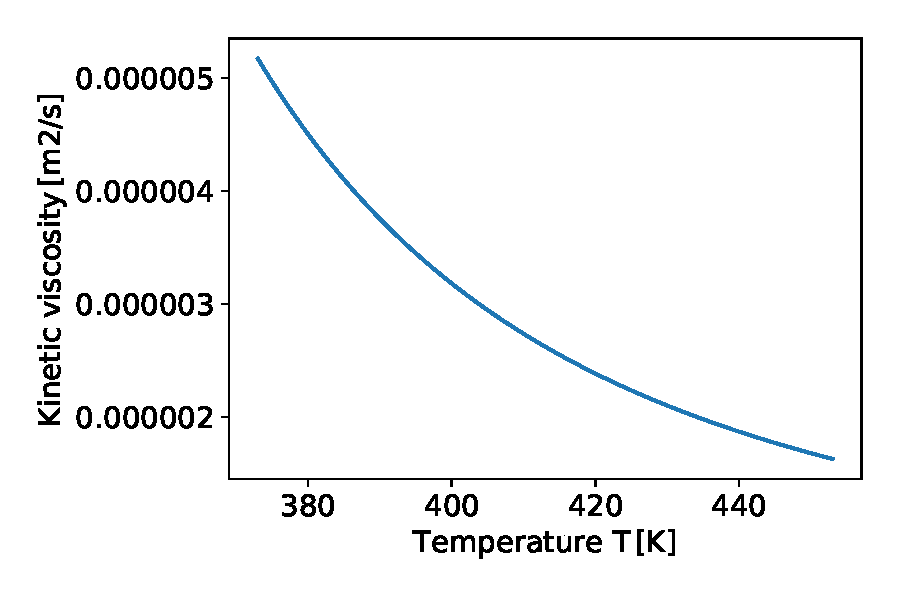
\includegraphics[width=0.48\textwidth,natwidth=190,natheight=210]{fig/kinetic_viscosity.pdf}
 \vspace{-1zh}
 \caption{Kinetic viscosity nu, $\rm m^{2}/s$}\label{kinetic_viscosity}
\end{minipage}
\hfill
\begin{minipage}{0.48\linewidth}
 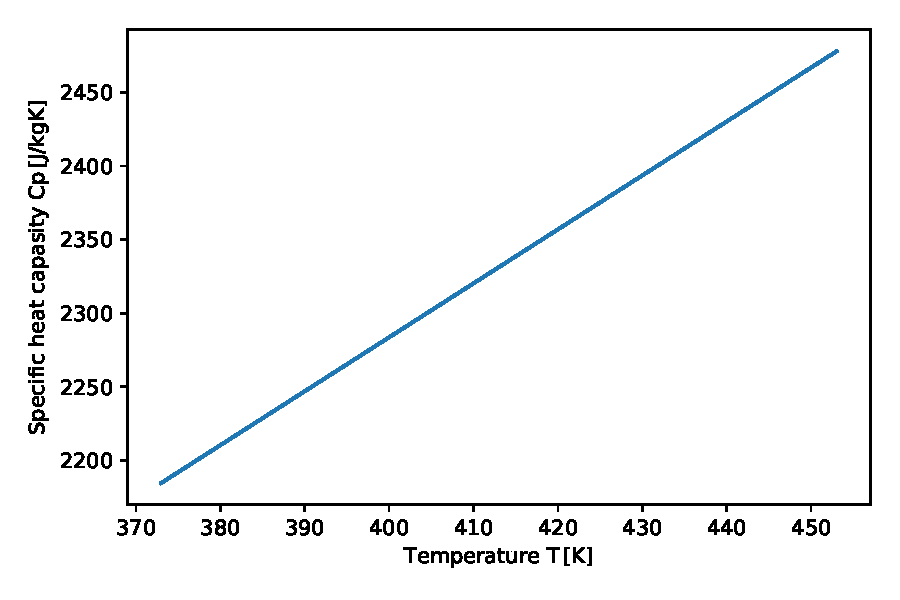
\includegraphics[width=0.48\textwidth,natwidth=190,natheight=210]{fig/heat_capacity.pdf}
 \vspace{-1zh}
 \caption{Heat capacity Cp, $\rm J/kgK$}\label{heat_capacity}
\end{minipage}
\vspace{2zh}
\end{figure}

\begin{figure}[h]
\begin{minipage}{0.48\linewidth}
 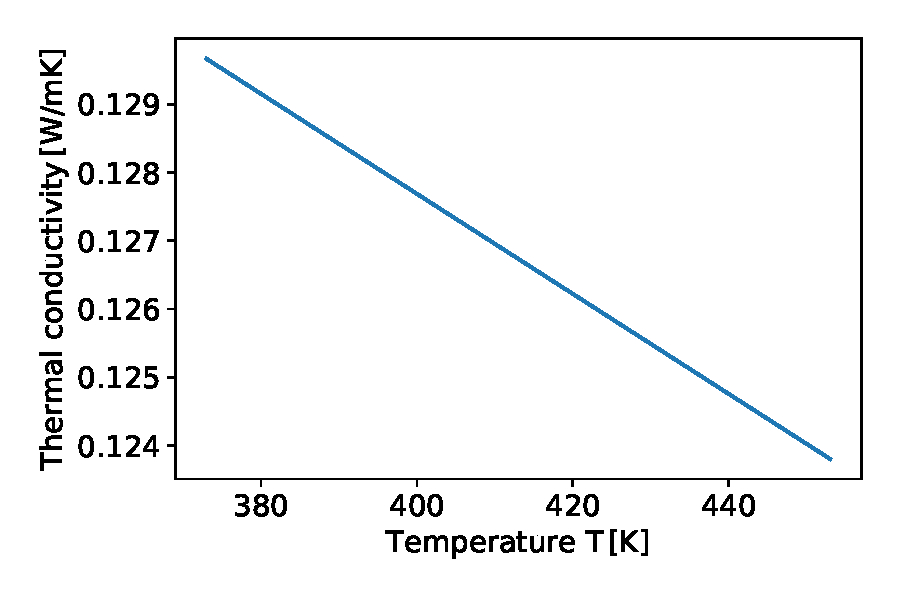
\includegraphics[width=0.48\textwidth,natwidth=190,natheight=210]{fig/thermal_conductivity.pdf}
 \vspace{-1zh}
 \caption{Thermal conductivity, $\rm W / m k$}\label{thermal_conductivity}
\end{minipage}
\hfill
\begin{minipage}{0.48\linewidth}
 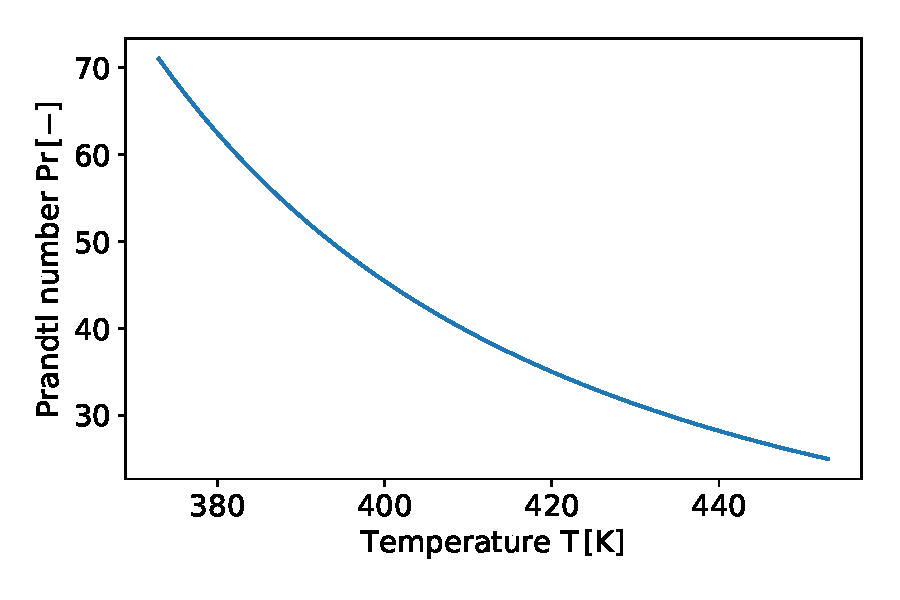
\includegraphics[width=0.48\textwidth,natwidth=190,natheight=210]{fig/prandtl_number.pdf}
 \vspace{-1zh}
 \caption{Prandtl number Pr, -}\label{prandtl_number}
\end{minipage}
%\vspace{-2zh}
\end{figure}

%\begin{figure}[h]
% \begin{minipage}{0.48\linewidth}
% \begin{center}
%   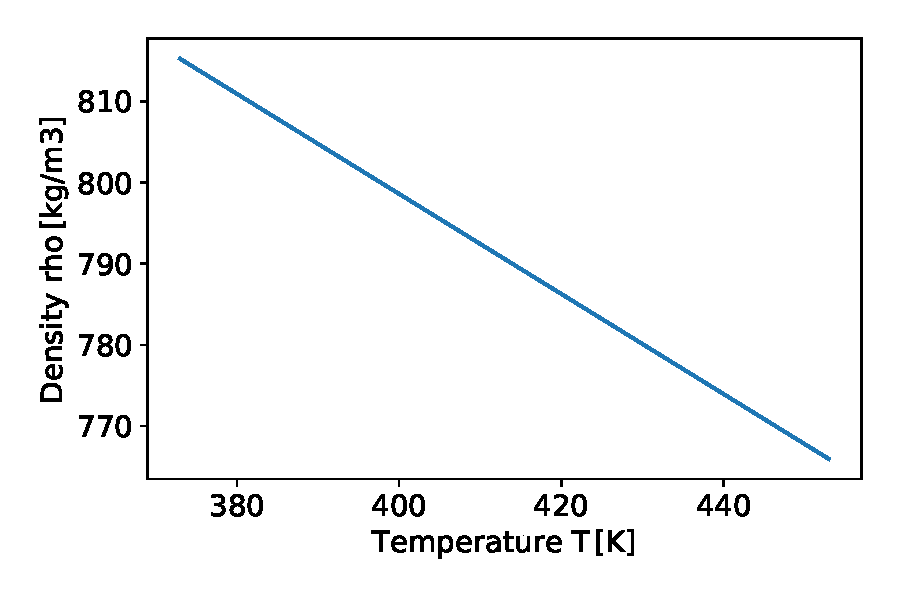
\includegraphics[width=0.47\textwidth,natwidth=280,natheight=300]{fig/density_rho.pdf}
%  \end{center}
%  \caption{$q=50\,\rm kW/m^2$ \cite{Inoue2016}}\label{HeatFlux=50k}
% \end{minipage}
% \hfill
% \begin{minipage}{0.48\linewidth}
% \begin{center}
%   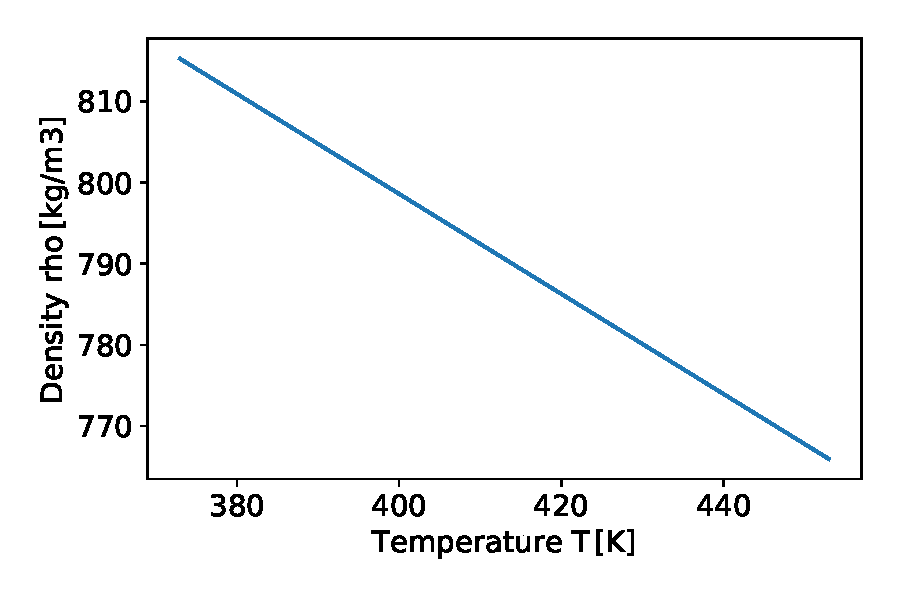
\includegraphics[width=0.47\textwidth,natwidth=610,natheight=642]{fig/density_rho.pdf}
%  \end{center}
%  \caption{$q=50\,\rm kW/m^2$ \cite{Inoue2016}}\label{HeatFlux=50k}
% \end{minipage}
% \vspace{-2zh}
%\end{figure}


\section{Calucuration Flow}
Material properties are temperature-dependent function.
Therefore, those were fitted to the data.
%including post processing

\section{Correlations}
Skinf friction coefficient for laminar flow is descrived following equation.
\begin{equation}
C_{f,lam}=\frac{16}{Re_{b}}
\end{equation}
Konakov(1954) showed skin friction coefficient for turbulent flow.
\begin{equation}
C_{f,turb}=0.25(1.8log(Re_{b})-1.5)^{-2}
\end{equation}
Note that these skin friction coefficient just suitable for no-heating condition, constant fluid properties.
In this thesis, we provide heat to the pipe.
Therefore, the fluid properties change depend on the temperature.

From general dimensional analysis, Nusselt number represents function of Reynolds number (Re) times Prandtl number (Pr) as following equation.
\begin{equation}
Nu=\alpha \cdot Re^{\pi_{\beta}}\cdot Pr^{\pi_{\gamma}}\label{Nu_dimensional}
\end{equation}
Here, factors $\alpha$, $\beta$ and $\gamma$ are constant value depend on flow regime and calcurated from numerical experimental results.
Gunienski\cite{Gnienlinski2010} showed correlations for each flow regime laminar and turbulent, respectively.
Gunienski\cite{Gnienlinski2010} showed calculation method for laminar flow.
\begin{equation}
Nu_{lam}=(3.66^{3}+0.7^{3}+(1.615(Re_{b}Pr_{b}\frac{d_{i}}{L})^{1/3})^{3})^{1/3}\label{Nu_laminar}
\end{equation}
%The range 0.1<<Pr_{b}<<1000, 10^{4}<<Re_{b}<<10^{6}.
Gunienski\cite{Gnienlinski2010} showed calculation method for turbulent flow.
\begin{equation}
Nu_{turb}=\frac{\frac{C_{f}}{2Re\cdot Pr_{b}}}{1+12.7 \sqrt{\frac{C_{f}}{2}}(Pr_{b}^{2/3}-1)}\cdot (\frac{Pr_{b}}{Pr_{w}})^{0.11}
%Nu_{turb}=\frac{\frac{C_{f}}{2\cdot Re\cdot Pr_{b}}{(1+12.7\frac{C_{f}}{2}}\cdot (Pr^{\frac{2}{3}}-1)}\cdot(1+(\frac{d_{h}}{l})^{\frac{2}{3}})\label{Nu_turblent}
\end{equation}
The range is
\begin{equation}
0.1<<Pr_{b}<<1000, 10^{4}<<Re_{b}<<10^{6}.
\end{equation}
He presented transitional flow as a liner interpolation between turbulent and laminar flow.
\begin{equation}
Nu_{m}=(1-r)Nu_{m,lam}+rNu_{m,turb}
\label{Nu_m}
\end{equation}
\begin{equation}
r=\frac{Re_{b}-2300}{10^{4}-2300}
\end{equation}

\section{State-of-the-art}
The presentaly considerd oil is Shell Heat Transfer oil S2.
The result show good agreement with correlations.

\section{Scientific problems and interests issues}
\begin{enumerate}
  \item Fluid properties\\
  Density, heat conductivity, specific heat transfer Cp, nu, mu, Pr are all varies with temperature.
  It is difficult to keep high Pramdlt number and transitional Reynolds number.
  For example, as enhance cooling, temperature decrease, statics viscosity increase.
  As a result, Pr increase and Re decrease.
  The ways to control Pr and Re are pointed above.
  Pr and Re are related each other and it it difficult to maintain the value that we want to measure.
  \item Temperature calibration\\
  There are two kinds of temperature measurement, Pt-100 and thermocouples.
  Thermocouples are calibrated by Pt-100 because Pt-100 is accurate enough.
  When we calibrate, the thermocouple temperature is always lower than Pt-100.
  \item Fully developed length\\
  \item 3 parameters(Nu,Re,Pr)\\
  The aim is to set Prandlt number level and vary the Reynolds number.
  There are only two parameters to descrive the correlation between Nusselt number and Reynolds number.
  The only choice is to take average Prandlt number.
  \item As increasing pump power, increasing flow speed and decreasing Pr number vary with heat transfer rate.\\
  Increasing pump power = Flow speed(Re) + Heat transfer rate(Pr) + Enthalpy\\
  Calcurating enthalpy, I guess it would be easy to control pump power.
  \item Thermal contact resistant of the capton tape which is connected with pipe and thermocouple.
  
  \item Turbulent intencity
  \item Slliped Knudsen number
  \item Corrilation between enthalpy and temperature profile
  
  \item Oil properties depend on long-distance time
  \item Outside temperature unceirtenty
  \item Pipe surface roughness
  \item Low temperature cooling
  \item Temperature genelation(round?)
\end{enumerate}

%Many studies have pointed out that heat transfer coefficient vary depending on the type of flow: laminar, transition and turbulent.
%Gnienlinski\cite{Gnienlinski2010} showed calculation method for laminar heat transfer coefficient of two kinds of boundary conditions. (I) Constant wall temperature (UWT) and (I\hspace{-.1em}I) Constant heat flux (UHF).
%
%\begin{equation}
%Nu_{lam}=\sqrt[3]{Nu_{1}^{3}+b^{3}+(Nu_{2}-b)^{3}+Nu_{3}^{3}}\label{Nu_laminar}
%\end{equation}
%For a cylindical pipe flow, the factor b is equal to b=3.
%\\For fully developed thermal and hydrodynamic flow the heat transfer coeficient.
%Graetz number define as Gz.
%\begin{equation}
%Nu_{1}=3.66
%\end{equation}
%\begin{equation}
%Nu_{2}=1.615\cdot \sqrt[3]{Gz}
%\end{equation}
%\begin{equation}
%Nu_{3}=\sqrt[6]{\frac{2}{1+22\cdot Pr}}\cdot Gz
%\end{equation}
%For a constant heat flux (UHF) over the heat transfer surface, those equations take the effect of the thermal boundary condition at heat transfering surface into account.
%\begin{equation}
%Nu_{1}=4.364
%\end{equation}
%\begin{equation}
%Nu_{2}=1.953\cdot \sqrt[3]{Gz}
%\end{equation}
%\begin{equation}
%Nu_{3}=0.924\cdot Pr^{\frac{1}{3}}\cdot \sqrt{Re\cdot \frac{d_{h}}{l}}
%\end{equation}
%Petukhvov and Kirillov\cite{Petukhov1958} showed calculation method for turbulent flow.
%\begin{equation}
%Nu_{turb}=\frac{\frac{\xi}{8}\cdot Re\cdot Pr}{(1+12.7\cdot \frac{\xi}{8})^{0.5}\cdot (Pr^{\frac{2}{3}}-1)}\cdot(1+(\frac{d_{h}}{l})^{\frac{2}{3}})\label{Nu_turblent}
%\end{equation}
%\begin{equation}
%\xi=(1.8\log{10}Re-1.5)^{-2}
%\label{Nu_turblent_xi}
%\end{equation}


%Bertsche et al,\cite{Bertsche2016} focused on reliable prediction of heat transfer coefficient for transitional flows.
%In their study, Bertsche et al, showed experimental heat transfer coefficients for Reynolds number $500 < Re < 23000$ and Prandtl number $7 < Pr < 41$.

\section*{Acknowledgment}
%I would like to thank my thesis advisors Prof. Helfried Steiner and Prof. Guenter Brenn of the Institute of Fluid Mechanics and Heat Transfer at Graz University of Technology.
%%The door to Prof. Shirai of Mechanical Engineering department at Shibaura Institute of Technology was always support my studying abroad.
%I am also grateful to Dr. Shirai of Mechanical Engineering department at Shibaura Institute of Technology.
%I am extremely thankful and indebted to him for sharing his experiments.
%I would also like to thank Dr. Tange allowed my studying in Graz, Austria.


\begin{thebibliography}{00}
 \bibitem{Frank} Frank P. Incropera, David P. DeWitt, ``Fundamentals of Heat and Mass Transfer,'' 4th edition., WILEY, 1996.
 \bibitem{Gnienlinski2010} V. Gnienlinski, ``Heat Transfer in Laminar Flow,'' VDI Heat Atlas, second ed., Springer Verlag, 2010 (Chapter Ga 1-7), Section 3.
 \bibitem{Petukhov1958} B.S. Petukhov, V.V. kirillov, Teploenergetika 4 (1958) 91-98.
 \bibitem{Bertsche2016} Dirk Bertsche, Paul Knipper, Thomas Wetzel, ``Experimental investigation on heat transfer in laminar, transitional and turbulent circular pipe flow,'' International Journal of Heat Transfer, 95 (2016) 1008-1018.
\bibitem{Rorenzo2019} Rorenzo, ``Title of paper if known,'' unpublished, 2019.
% \bibitem{b5} R. Nicole, ``Title of paper with only first word capitalized,'' J. Name Stand. Abbrev., in press.
% \bibitem{b6} Y. Yorozu, M. Hirano, K. Oka, and Y. Tagawa, ``Electron spectroscopy studies on magneto-optical media and plastic substrate interface,'' IEEE Transl. J. Magn. Japan, vol. 2, pp. 740--741, August 1987 [Digests 9th Annual Conf. Magnetics Japan, p. 301, 1982].
% \bibitem{b7} M. Young, The Technical Writer's Handbook. Mill Valley, CA: University Science, 1989.

%\bibliography{junsrt}
%\bibliography{project_forced_convective@Graz.bib}

\end{thebibliography}
%\vspace{12pt}
%\color{red}
%IEEE conference templates contain guidance text for composing and formatting conference papers. Please ensure that all template text is removed from your conference paper prior to submission to the conference. Failure to remove the template text from your paper may result in your paper not being published.

\end{document}
